%\title{Project Report}
%
%%% Preamble
\documentclass[paper=a4, fontsize=11pt]{scrartcl}
\usepackage[T1]{fontenc}
\usepackage{fourier}

\usepackage[english]{babel}															% English language/hyphenation
\usepackage[protrusion=true,expansion=true]{microtype}	
\usepackage{amsmath,amsfonts,amsthm} % Math packages
\usepackage[pdftex]{graphicx}	
\usepackage{url}
\usepackage{hyperref}
\usepackage{graphicx}
\usepackage{wrapfig}
\usepackage[margin=0.75in]{geometry}

%%% Custom sectioning
\usepackage{sectsty}
\allsectionsfont{\centering \normalfont\scshape}


%%% Custom headers/footers (fancyhdr package)
\usepackage{fancyhdr}
\pagestyle{fancyplain}
\fancyhead{}											% No page header
\fancyfoot[L]{}											% Empty 
\fancyfoot[C]{}											% Empty
\fancyfoot[R]{\thepage}									% Pagenumbering
\renewcommand{\headrulewidth}{0pt}			% Remove header underlines
\renewcommand{\footrulewidth}{0pt}				% Remove footer underlines
\setlength{\headheight}{3.6pt}
\date{}


%%% Equation and float numbering
\numberwithin{equation}{section}		% Equationnumbering: section.eq#
\numberwithin{figure}{section}			% Figurenumbering: section.fig#
\numberwithin{table}{section}				% Tablenumbering: section.tab#


%%% Maketitle metadata
\newcommand{\horrule}[1]{\rule{\linewidth}{#1}} 	% Horizontal rule

\title{
		\vspace{-1in} 	
		\usefont{OT1}{bch}{b}{n}
		\normalfont \normalsize \textsc{Durham Computer Science} \\ [5pt]
		\horrule{0.5pt} \\[0.4cm]
		\huge Numerical Algorithms Assignment - LLLL76\\
		\horrule{2pt} \\[0.5cm]
		\vspace{-1in} 	
}

%%% Begin document
\begin{document}
\maketitle
\section{}
\subsection{Code Modifications}

\begin{wrapfigure}{r}{0.33\textwidth} %this figure will be at the right
    \centering
    \caption{Figure One}
    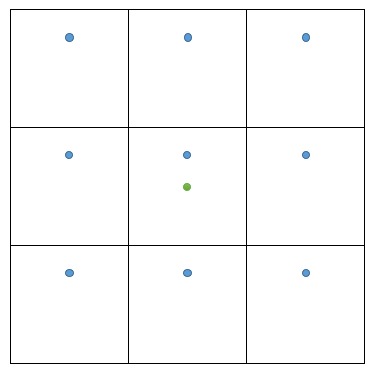
\includegraphics[width=0.33\textwidth]{9.png}
\end{wrapfigure}

Start with an arbitrary number of particles and time steps, using a random number generator each particle is given an x, y and z coordinate. The interaction will start by iterating through every particle in the simulation and also iterating through each "mirror" of the current particle that exists, and a part example of these mirrors is shown in figure 1, for each one calculating the euclidean distance from the current particle to each other particle and using this distance to calculate the force on the current particle, this will then be split into its constituent parts, x,y and z. After iterating through all other particles the forces in each direction are totalled to give the total force in each direction for a single particle, this will be done for all particles. The distance that each particle will travel is calculated using this force and the time step value, after all travel calculations are done, all particles will be moved. The only other feature of the simulation is periodic bounding, I had done this by modulo mathematics but this introduced a few issues, so decided that comparison was faster and more reliable. The comparisons are done is such a way that they are used every time a particle has its coordinates changed. The particles will have their coordinates changed after all the forces have been calculated for every particle, this improves accuracy as the first particle doesn't have it's coordinates changed then this new position is used for the other particles in the simulation.

\subsection{Improvements}
Whilst iterating through each particle pair, the shortest distance between any particle pair is stored, this will be used to calculate the time step, initially the time step is set to the minimum possible value. A variable time step is used because of the tendency of particle to accelerate together, due to the implementation it will do this in jumps, if the time step is too large then the particle will pass each other without the particles ever being close enough to repel and will thus not be an accurate model. The way that I calculate the time step is based on experimental data, I set two particles at closer and closer distances together and set a time step that I thought was acceptable based on para view play speed, I then created a stepped time step such that if the shortest distance between any two particle pairs was between two thresholds then the time step would change based on this, and when the distance dropped bellow the lower threshold then the time step would change, this was jerky with the particles accelerating together then coming to a halt as the time step changed, this was done several times as the distance between any two particles lessened. To overcome the stepping I plotted threshold/time step points and used a line of best fit to give me the equation of the line that would best fit the thresholds I had found. The equation happened to be the $shortest distance^{2.7469} * 10^{10}$. This was proved to be accurate above a distance of 0.00015 by experimentation, at this point just the minimum distance was used as the time step, this allows high accuracy at very short distances. \\
An improvement that I did make was to reduce the number of euclidean distances calculated was to use force calculated on the current particle on the other particle as well, this has the affect of halving the number of euclidean distance calculation and force calculations that have been done. The way I have implemented wrap around forces is to iterate through the 27 or 7 different dimensions, dependent on the file, I have run both to test run times. Each of the dimensions corresponds to an index in an array that stores the change in coordinates that a particle would have to go through to translate to the corresponding mirror particle, this mirror particle is then used to calculate the force on the current particle from the wrap around in that direction. If this were to be made more accurate then the wrap around would be done for an infinite number of wrap around forces, this is infeasible so I have done it for both 27 and 7.

\section{}

Per setup: Result is correct qualitatively
(2 marks), convergence rate is
reasonable w.r.t. time step size (4
marks), description is accurate and
precise (2 marks), results are
interpreted correctly (2 marks). 

\subsection{Non-Wrap Around Test}

Given two particles and a non variable time step, with the two particles having coordinated of (0.4,0.5,0.5) and (0.6,0.5,0.5) respectively. Due to the implementation the particles will have the force calculated on each one then in a separate loop, they have their coordinates changed, this will results in "jumping" taking place. At high time steps these jumps will be so large that when the two particles get closer together and the forces increase then they will "jump" over one another and the simulation will be inaccurate. the sign will flip but only after the particles have passed one another. At lower time steps, if the particles start at 0.4 and 0.6 then they do not "jump" far enough for it to be noticeable in Paraview, however if they are initially set so that the distance between the two is lessened significantly the particles will oscillate around the 0.5 value as is expected. The two ways I have found to remove this issue are either variable time steps or normalizing the values of a and s to 0.1 not $10^-5$. The latter of which is shown in both youtube links bellow.\\
Variable time steps adds a fair amount of additional computation but I thought it was necessary for an accurate simulation, so this is the one that I have implemented in both step one and step three.

\url{https://www.youtube.com/watch?v=YEhfEQuVO8U}

\subsection{Wrap Around Test}

Given two particles and a non variable time step, with two particles having coordinates of (0.1,0.5,0.5) and (0.9,0.5,0.5) respectively. This will have same characteristics as the previous test but the centre of oscillation will be 0.0. This is caused by the wrap-around forces, which act in the 0.2 gap that exists between the particles in the X wrap around direction. The normalized version of this is shown in the youtube link bellow.

\url{https://www.youtube.com/watch?v=xx4zs1EaRf0}

\subsection{Results and Observations}

\centering
\begin{tabular}{ |p{7.5cm}||p{7.5cm}|  }
 \hline
 \multicolumn{2}{|c|}{Time Taken} \\
 \hline
 Number of particles & Time taken for 200 time steps (seconds)\\
 \hline
 10 & 3.2 \\
 100 & 361 \\
 1000 & 37681 \\
 10000 & 3781620 \\
 100000 & 377118000 \\
 \hline
\end{tabular}

\section{}

Brief description of step 3 is precise
and clear (5 marks). Runtime impact is
experimentally determined and
explanation for runtime behaviour is
given (5 marks). Error is determined
through Taylor expansion (5 marks). All
experiments are rerun and results are
discussed (5 marks).

\subsection{Measure of Correctness}

To prove correctness I have re-run the tests in step two and compare the results. Due to the cut off radii that in present in both data structures that I have researched, namely: cell lists and Verlet lists, the cut off is a distance around every particle outside of which no particle can apply a force on the current particle, both the simulations run and neither of the particles move due to the recommended cut off radii being so much smaller that the distance between the two particles in any of the simulations. In the simulations of higher numbers of particles the particle density increased significantly meaning that particles were more likely to be within the cut off radius and thus an interaction occurred with in turn caused more interactions to occur and this continued at a fairly set rate for the duration I have simulated. With higher numbers of particles the simulation is more accurate but at lower numbers of particles there is a high chance, due to the very small recommended cut off radius, that nothing will happen. A way to counter the inaction of particles is to increase the cut off radius, this would be beneficial for lower numbers of particles because they would interact however for higher number of particles the idea of there data structures are to minimise the computation time by reducing the number of calculations done, with a large cut off radius and many particles the reduction in number of calculations is very small whilst still being, in comparison to step one, inaccurate. The ideal cut off radii for varying numbers of particles changes significantly to balance reduction in computation time and reduction in accuracy. At a high numbers of particles the simulation is still reasonably correct with the low cut off radius, at lower numbers of particles and the low cut off radius it is not reasonably correct. 

\subsection{Data Structure}

The data structure I decided to use is called a Verlet list, this is a data structure that, for each particle a list of nearby particles are stored that are within some pre-decided cut off radius. This list is updated regularly, in this simulation it is done every set number of time steps, on the time steps that the list isn't updated each particle will iterate through the the list that corresponds to it and only the particles in this list will be able to apply a force on the current particle. In my implementation we also need another list for each particle that will store the mirror of the particle that is close enough to the current particle to cause the force so as to have the correct mirror of the particle. When the list is to be updated each particle will iterate through all 27 mirrors of the other particles and store any instances of this that are within the cut off radius. 

\subsection{Results}

\centering
\begin{tabular}{ |p{5cm}||p{5cm}|p{5cm}|}
 \hline
 \multicolumn{3}{|c|}{Time Taken} \\
 \hline
 Number of particles & Time taken for 200 time steps (seconds, part one) & Time taken for 200 time steps (seconds, part three)\\
 \hline
 10 & 3.2 & 0.029 \\
 100 & 361 & 29.90 \\
 1000 & 37681 & 2920 \\
 10000 & 3781620 & 293920 \\
 100000 & 377118000 & 29872000\\
 \hline
\end{tabular}

\subsection{Taylor Expansion}

The error introduced due to step three is equal to the change in position that would have occurred due to a particle at the cut off point. This is based on the fact that if a particle was present on the cut off radius, step one would calculate the change in coordinates that would occur due to the force exerted on the particle whilst step three would not have a force exerted on the particle due to the cut off, and thus not have an acceleration and thus not have a speed and thus not change its coordinates the error introduced is the distance that a particle would have travelled had the cut off radius not been introduced. This is equal to the force that would have been applied to the particle by a particle with radius equal to the cut off distance multiplied by the time step squared.\\
\center
$f(r) = 4a((12 * s^(12) / r^(13)) - (6 * s^6 / r^7))$\\
where a = s = $10^-5$\\
and r = $2.5 * s$\\
$f(r) = 4 * 10^-5((12 * 10^-5^12/(2.5 * 1-^-5)^13) - (6 * 10^-5^6 / (2.5 * 10^-5)^7))$\\
error = $f(r) * t^2$\\
$f(r)$ roughly equals $0.039$\\
error roughly equals $0.039 * t^2$\\


%%% End document
\end{document}